\begin{definitionbox}{Definition --- Restricted Distance}
\begin{definition}[Restricted Distance]\label{def:metric-restricted-distance}
Let \(Y\) be a metric space, and let \(X\subseteq Y\).  The
\emph{restricted distance} on \(X\) is the function
\[
  d_X(x,y):=d_Y(x,y)
\]
for all \(x,y\in X\).
\end{definition}
\end{definitionbox}

\begin{remark*}[Standard quantified statement]
\[
\forall x,y\in X{:}\quad d_X(x,y)=d_Y(x,y).
\]
\end{remark*}

\begin{remark*}[Predicate reading]
\[
d_X=d_Y|_{X\times X}
\]
means that the distance assigned inside the subset is the ambient distance
restricted to pairs of points in the subset.
\end{remark*}

\begin{remark*}[Interpretation]
Restriction keeps the same numerical distances but only allows points from
the subset.  It is the basic mechanism by which a subset inherits metric
structure from an ambient metric space.
\end{remark*}

\begin{figure}[htbp]
\centering
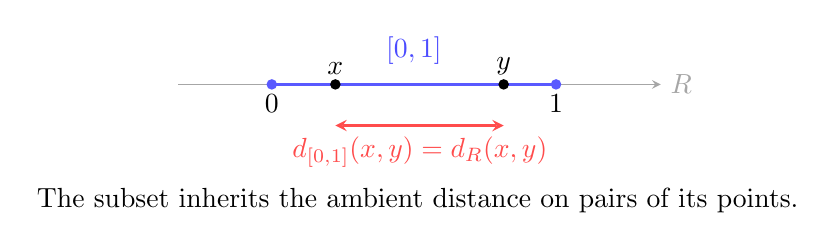
\begin{tikzpicture}[scale=0.95,>=stealth]
  \draw[->,gray!70] (-0.25,0) -- (6.2,0) node[right] {\(\mathbb{R}\)};
  \draw[blue!65,very thick] (1.0,0) -- (4.8,0);
  \fill[blue!65] (1.0,0) circle (2pt);
  \fill[blue!65] (4.8,0) circle (2pt);
  \node[below] at (1.0,0) {\(0\)};
  \node[below] at (4.8,0) {\(1\)};
  \node[blue!70] at (2.9,0.45) {\([0,1]\)};

  \fill[black] (1.85,0) circle (2pt);
  \fill[black] (4.1,0) circle (2pt);
  \node[above] at (1.85,0) {\(x\)};
  \node[above] at (4.1,0) {\(y\)};
  \draw[<->,red!70,thick] (1.85,-0.55) -- (4.1,-0.55);
  \node[red!70] at (2.98,-0.9) {\(d_{[0,1]}(x,y)=d_{\mathbb{R}}(x,y)\)};

  \node[align=center] at (2.95,-1.55)
    {The subset inherits the ambient distance on pairs of its points.};
\end{tikzpicture}

\caption{A metric subspace keeps the ambient distance between points of the
subset.  The closed unit interval inherits its distance from the real line by
restriction.}
\label{fig:restricted-distance-subspace}
\end{figure}

\LeanFormalizes{def:metric-restricted-distance}{lra-lean}{LRA.VolumeIV.MetricSpaces.SubSuperSpaces.Basic}{restrictedDistance}{statement}

\begin{dependencies}
\begin{itemize}
  \item \hyperref[def:metric-space]{Definition: Metric Space}
\end{itemize}
\end{dependencies}

\begin{definitionbox}{Definition --- Metric Subspace}
\begin{definition}[Metric Subspace]\label{def:metric-subspace}
Let \(Y\) be a metric space and let \(X\subseteq Y\).  A metric space carried
by \(X\) is a \emph{metric subspace} of \(Y\) when its metric is the
restriction of the ambient metric on \(Y\) to \(X\times X\).
\end{definition}
\end{definitionbox}

\begin{remark*}[Standard quantified statement]
\[
  \forall x,y\in X{:}\quad d_X(x,y)=d_Y(x,y).
\]
\end{remark*}

\begin{remark*}[Predicate reading]
\[
X\text{ is a metric subspace of }Y
\]
means that \(X\), with its own metric, carries exactly the distance inherited
from the ambient metric space \(Y\).
\end{remark*}

\begin{remark*}[Interpretation]
A metric subspace is not just a subset.  It is a subset whose metric agrees
with the ambient distance on every pair of its points.
\end{remark*}

\LeanFormalizes{def:metric-subspace}{lra-lean}{LRA.VolumeIV.MetricSpaces.SubSuperSpaces.Basic}{MetricSubspaceDefinition}{statement}
\LeanFormalizes{def:metric-subspace}{lra-lean}{LRA.VolumeIV.MetricSpaces.SubSuperSpaces.Basic}{IsMetricSubspace}{statement}

\begin{dependencies}
\begin{itemize}
  \item \hyperref[def:metric-space]{Definition: Metric Space}
  \item \hyperref[def:metric-restricted-distance]{Definition: Restricted Distance}
\end{itemize}
\end{dependencies}

\begin{definitionbox}{Definition --- Metric Superspace}
\begin{definition}[Metric Superspace]\label{def:metric-superspace}
Let \(X\) be a metric subspace of a metric space \(Y\).  Then \(Y\) is called
a \emph{metric superspace} of \(X\).
\end{definition}
\end{definitionbox}

\begin{remark*}[Standard quantified statement]
\[
Y\text{ is a metric superspace of }X
\Longleftrightarrow
X\text{ is a metric subspace of }Y.
\]
\end{remark*}

\begin{remark*}[Interpretation]
Subspace and superspace describe the same restriction relation from opposite
directions.  The subspace is the subset with the inherited metric, while the
superspace is the ambient metric space from which the distance is inherited.
\end{remark*}

\LeanFormalizes{def:metric-superspace}{lra-lean}{LRA.VolumeIV.MetricSpaces.SubSuperSpaces.Basic}{MetricSuperspaceDefinition}{statement}
\LeanFormalizes{def:metric-superspace}{lra-lean}{LRA.VolumeIV.MetricSpaces.SubSuperSpaces.Basic}{IsMetricSuperspace}{statement}

\begin{dependencies}
\begin{itemize}
  \item \hyperref[def:metric-subspace]{Definition: Metric Subspace}
\end{itemize}
\end{dependencies}

\begin{propositionbox}{Proposition}
\begin{proposition}[The Closed Unit Interval Is a Metric Subspace of the Real Line]
\label{prop:closed-unit-interval-metric-subspace}
The closed unit interval \([0,1]\), with the distance inherited from
\(\mathbb{R}\), is a metric subspace of the real line.
\hyperref[prf:closed-unit-interval-metric-subspace]{\textit{Go to proof.}}
\end{proposition}
\end{propositionbox}

\begin{remark*}[Standard quantified statement]
\[
[0,1]\subseteq\mathbb{R}
\quad\text{with inherited distance is a metric subspace of }\mathbb{R}.
\]
\end{remark*}

\begin{remark*}[Interpretation]
Distances between points of \([0,1]\) are exactly the same whether those
points are viewed inside the interval or inside the real line.
\end{remark*}

\LeanFormalizes{prop:closed-unit-interval-metric-subspace}{lra-lean}{LRA.VolumeIV.MetricSpaces.SubSuperSpaces.Basic}{closedUnitInterval_isMetricSubspace}{checked}

\begin{dependencies}
\begin{itemize}
  \item \hyperref[def:metric-subspace]{Definition: Metric Subspace}
  \item \hyperref[def:real-line-euclidean-distance]{Definition: Euclidean Distance on \(\mathbb{R}\)}
\end{itemize}
\end{dependencies}

\begin{propositionbox}{Proposition}
\begin{proposition}[The Real Line Is a Metric Superspace of the Closed Unit Interval]
\label{prop:real-line-metric-superspace-closed-unit-interval}
The real line is a metric superspace of the closed unit interval \([0,1]\)
with its inherited metric.
\hyperref[prf:real-line-metric-superspace-closed-unit-interval]{\textit{Go to proof.}}
\end{proposition}
\end{propositionbox}

\begin{remark*}[Standard quantified statement]
\[
\mathbb{R}\text{ is a metric superspace of }[0,1].
\]
\end{remark*}

\begin{remark*}[Interpretation]
The real line is the ambient metric space from which the closed unit interval
inherits its distance.
\end{remark*}

\LeanFormalizes{prop:real-line-metric-superspace-closed-unit-interval}{lra-lean}{LRA.VolumeIV.MetricSpaces.SubSuperSpaces.Basic}{real_isMetricSuperspace_closedUnitInterval}{checked}

\begin{dependencies}
\begin{itemize}
  \item \hyperref[def:metric-superspace]{Definition: Metric Superspace}
  \item \hyperref[prop:closed-unit-interval-metric-subspace]{Proposition: The Closed Unit Interval Is a Metric Subspace of the Real Line}
\end{itemize}
\end{dependencies}
